
\documentclass[conference]{IEEEtran}

\usepackage{amsmath}
\usepackage{amssymb}
\usepackage{graphicx}
\usepackage{booktabs}
\usepackage{float}
\usepackage{hyperref}
\usepackage{listings}
\usepackage{xcolor}
\usepackage{url}
\usepackage{listings}

\lstset{
    basicstyle=\ttfamily\footnotesize,
    breaklines=true,
    frame=single,
    numbers=left,
    numberstyle=\tiny,
    captionpos=b,
    columns=fullflexible
}

\title{Algorithmic Applications of Network Flow and NP-Hard Optimization}

\author{
\IEEEauthorblockN{Pradhyuman Singh Shekahwat}
\IEEEauthorblockA{COT5405 -- Project 2}
}

\begin{document}

\maketitle

\begin{abstract}
This project examines two real-world optimization problems through
algorithmic techniques. The first models water distribution as a
maximum-flow problem. The second models cloud workload consolidation
as a Bin Packing problem, establishing its computational hardness and
evaluating a greedy heuristic experimentally.
\end{abstract}

\section{Introduction}

This paper investigates two optimization problems and their
algorithmic formulations. The first problem is water distribution
through a capacitated network, formulated as a maximum-flow problem.
The second is cloud workload consolidation, formulated as a Bin
Packing problem.

Water distribution infrastructure must transport available
water through networks whose transmission capacities
constrain the amount that can reach downstream consumers.
Capacity-constrained allocation provides a useful abstraction
for studying how available supply can be distributed through
a network \cite{epa_distribution}. In this project, the hydraulic system is simplified
to a capacitated directed graph, allowing the allocation
objective to be studied using maximum-flow techniques.

Cloud computing infrastructure must allocate workloads
to physical or virtualized resources while respecting
resource limits. Consolidating workloads can reduce the
number of servers required in a simplified allocation
setting \cite{kubernetes_resources}. This project models each workload as a one-dimensional
item and each server as a fixed-capacity bin, isolating the
computational challenge of resource consolidation from
additional scheduling constraints.

% Report-ready section for the Network Flow component.
\section{Water Distribution as a Maximum-Flow Problem}
\label{sec:water-flow}

\subsection{Problem abstraction}
Let the physical water-distribution system be a directed graph
$G=(V,E)$, where each pipe $(u,v)\in E$ has a nonnegative capacity
$c(u,v)$. Let $P\subseteq V$ be supply nodes, with available supply
$s(p)\ge 0$, and let $D\subseteq V$ be demand nodes, with demand cap
$d(z)\ge 0$. The goal is to maximize the total water delivered to demand
nodes while respecting pipe capacities, supply limits, and demand limits.
This abstraction models capacity-constrained allocation; it does not model
hydraulic pressure, head loss, pipe dynamics, or water quality.

\subsection{Reduction construction}
Construct a flow network $G'=(V',E')$ by introducing a super-source $S$
and a super-sink $T$. Set $V'=V\cup\{S,T\}$. Retain every physical
pipe $(u,v)\in E$ with capacity $c(u,v)$. For each supply node $p\in P$,
add an edge $(S,p)$ with capacity $s(p)$. For each demand node $z\in D$,
add an edge $(z,T)$ with capacity $d(z)$. Run a maximum-flow algorithm
from $S$ to $T$ in $G'$.

\subsection{Correctness proof}
We show that feasible allocations in the original abstraction correspond
to feasible flows in $G'$ and that the objective value is preserved.

\paragraph{From a water allocation to a flow.}
Consider any feasible allocation of water through the physical network.
Assign the amount dispatched from each supply node $p$ to edge $(S,p)$.
For every physical pipe $(u,v)$, assign the amount of water sent through
that pipe to its corresponding edge in $G'$. Finally, assign the amount
received at demand node $z$ to edge $(z,T)$. Supply limits, pipe capacities,
and demand caps ensure that all edge-capacity constraints are satisfied.
At every intermediate node, conservation of water is exactly the flow
conservation constraint. Thus this assignment is a feasible $S$--$T$ flow.
Its value equals the total water delivered to the demand nodes.

\paragraph{From a flow to a water allocation.}
Conversely, take any feasible $S$--$T$ flow in $G'$. Interpret the flow
on each physical-pipe edge as the amount transported through that pipe,
the flow on $(S,p)$ as the amount drawn from supply node $p$, and the
flow on $(z,T)$ as the amount delivered to demand node $z$. Capacity
constraints enforce each pipe capacity, supply limit, and demand cap.
Flow conservation at intermediate vertices ensures that transported water
is balanced. The resulting allocation is therefore feasible in the original
abstraction, and its total delivered amount equals the flow value.

\paragraph{Optimality.}
The two mappings above preserve feasibility and objective value. Hence the
maximum possible water delivery in the abstraction is equal to the maximum
$S$--$T$ flow value in $G'$. A maximum-flow algorithm therefore produces
an optimal allocation for this model.

\subsection{Construction and algorithm complexity}
The transformation adds two vertices and at most $|P|+|D|$ edges beyond
the physical network. Its construction takes
$O(|V|+|E|+|P|+|D|)$ time under an adjacency-list representation.
The implementation then computes a maximum flow using Dinic's algorithm.
For a general directed network, Dinic's algorithm has the standard
$O(|V'|^2|E'|)$ worst-case bound. Since $|V'|=|V|+2$ and
$|E'|=|E|+|P|+|D|$, this is
$O((|V|+2)^2(|E|+|P|+|D|))$ for the constructed network.

% Report-ready section for the NP-completeness component.
\section{Cloud Workload Consolidation and Bin Packing}
\label{sec:binpacking}

\subsection{Problem abstraction}
Model each workload as an item with positive size $a_i$ and each identical
server as a bin of capacity $B$. The objective is to assign every item to
a bin without exceeding capacity and to minimize the number of bins used.
The decision version asks whether all items can be packed into at most $k$
bins. This is a simplified one-dimensional consolidation model; it does
not capture multi-dimensional resources, placement constraints, or runtime
migration costs.

\subsection{Membership in NP}
A certificate specifies the bin assigned to each item. In polynomial time,
a verifier checks that no item is assigned outside the proposed bins and
that the sum of item sizes in each bin does not exceed $B$. Therefore,
the decision version of Bin Packing is in NP.

\subsection{NP-hardness reduction from 3-Partition}
The complexity classification and reduction framework
follow the standard theory of NP-completeness
\cite{gareyjohnson}.
We reduce from 3-Partition, a strongly NP-complete problem. An instance
contains $3m$ positive integers $a_1,\ldots,a_{3m}$ and a positive
integer $B$ satisfying $\sum_i a_i=mB$ and
$B/4<a_i<B/2$ for every item. The question is whether the integers can
be partitioned into $m$ triples, each summing to $B$.

Construct a Bin Packing decision instance using the same $3m$ item sizes,
bin capacity $B$, and target number of bins $k=m$. This construction is
polynomial in the input size.

\paragraph{Forward direction.}
If the 3-Partition instance has a partition into $m$ triples each summing
to $B$, place each triple in one bin. Every bin has capacity $B$ and
exactly $m$ bins are used. Thus the constructed Bin Packing instance is
a yes-instance.

\paragraph{Reverse direction.}
Suppose the constructed Bin Packing instance can pack the items into at
most $m$ bins. The total item size is $mB$, while each bin has capacity
$B$. Consequently, all $m$ bins must be used and each must be filled to
capacity $B$. Since every item is strictly larger than $B/4$ and
strictly smaller than $B/2$, no bin can contain four or more items and
no bin can contain two or fewer items while being full. Each bin must
therefore contain exactly three items summing to $B$. These triples form
a valid solution to the 3-Partition instance.

\paragraph{Conclusion.}
The reduction preserves yes- and no-instances, so Bin Packing decision is
NP-hard. Combined with membership in NP, it is NP-complete. Because the
reduction is from strongly NP-complete 3-Partition, Bin Packing is also
strongly NP-hard in its optimization form.

\subsection{Greedy heuristic: First Fit Decreasing}
First Fit Decreasing is a classical bin-packing heuristic
studied in the literature on approximation algorithms
\cite{johnson1974}.
The implemented heuristic sorts items in nonincreasing order and places
each item into the earliest opened bin with sufficient remaining capacity.
If no opened bin fits, it opens a new bin. A segment tree stores the
maximum remaining capacity in each subtree and finds the leftmost bin
whose remaining capacity is at least the current item's size; the tree is
updated after each placement. The leftmost-fit query preserves First Fit
behavior while accelerating the search.

\subsection{Running time}
Sorting takes $O(n\log n)$. Each item requires a segment-tree query and
update, each taking $O(\log n)$, so placement takes $O(n\log n)$ total.
The overall running time is $O(n\log n)$ and the storage is $O(n)$.
First Fit Decreasing is a heuristic and does not guarantee an optimal
packing on every instance.

\section{Experimental Evaluation}

\subsection{Experimental Setup}

Each benchmark graph was generated using a fixed random
seed of 5405. A directed chain from the source to the sink
was included to guarantee a source-to-sink path. In addition,
approximately $4n$ random endpoint pairs were generated,
with endpoints ordered to produce forward edges and
self-loops discarded. Parallel edges were permitted.
Capacities were independently assigned from the integer
range 1 to 100. The graph was generated once for each
benchmark size and reused across the seven timed
executions. Graph construction was excluded from the
measured interval.

The experiments were conducted using C++ implementations of the
algorithms. The maximum-flow implementation uses Dinic's algorithm,
while the Bin Packing implementation uses First Fit Decreasing
(FFD) with a segment tree to accelerate bin selection.

The experiments were conducted on an Apple MacBook Pro
equipped with an Apple M1 Pro processor and running macOS
(Darwin 25.6.0) on the ARM64 architecture. The code was
compiled using Apple Clang 21.0.0
(compiler build clang-2100.1.1.101) with the CMake
Release configuration. The project build completed
successfully for the main executable, test executable,
and benchmark target.

\subsection{Maximum-Flow Experimental Results}

The maximum-flow implementation was evaluated on sparse directed
networks of increasing size. Each benchmark instance contained a
guaranteed source-to-sink path and additional edges generated
deterministically using a fixed random seed. The edge capacities
were drawn from the range 1 to 100. The graph generation procedure
was performed outside the timed execution.

Table~\ref{tab:flow_results} presents the median execution times.

\begin{table}[htbp]
\centering
\caption{Maximum-flow benchmark results}
\label{tab:flow_results}
\begin{tabular}{r r r}
\toprule
Vertices & Edges & Median (ms) \\
\midrule
1,000  & 4,996  & 1.14533 \\
2,000  & 9,997  & 1.91275 \\
4,000  & 19,994 & 4.25363 \\
8,000  & 39,993 & 19.46120 \\
12,000 & 59,999 & 39.40120 \\
\bottomrule
\end{tabular}
\end{table}

Figure~\ref{fig:flow_runtime} visualizes the measured runtime as
the network size increases.

\begin{figure}[htbp]
\centering
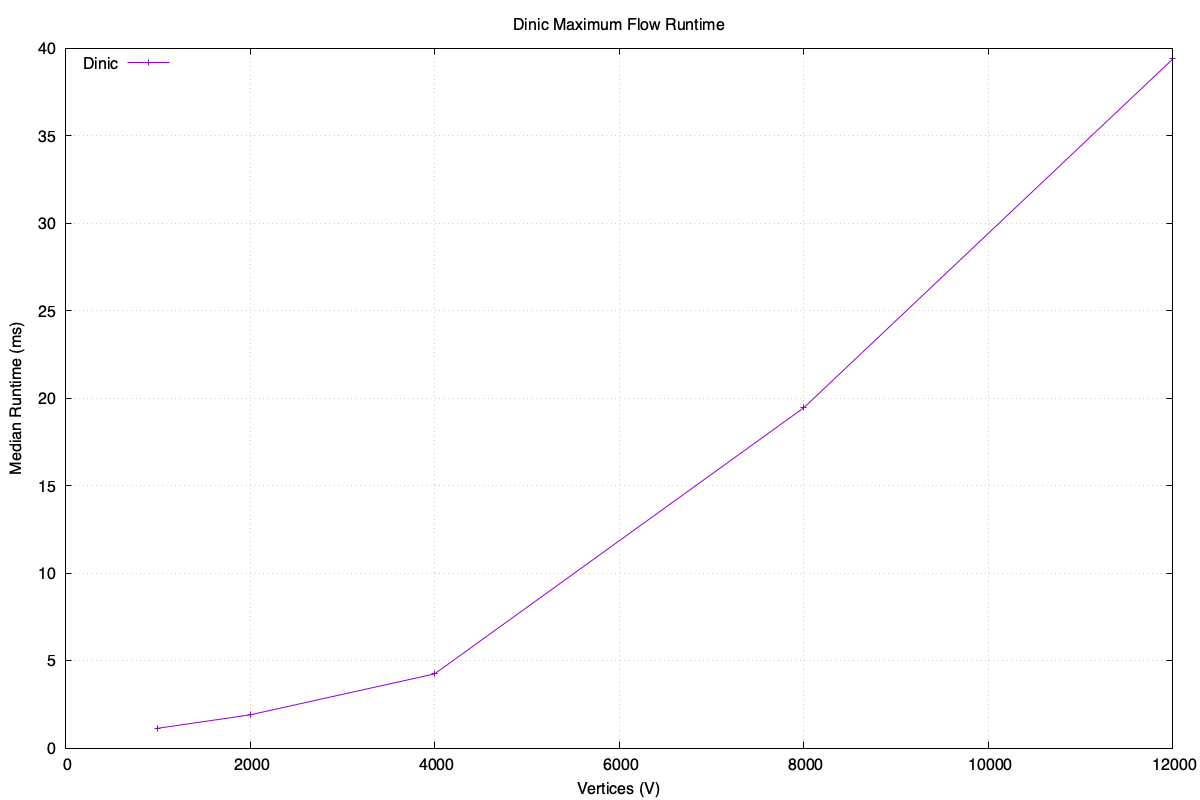
\includegraphics[width=\linewidth]{flow_runtime.png}
\caption{Measured runtime of Dinic's maximum-flow implementation
on sparse benchmark networks.}
\label{fig:flow_runtime}
\end{figure}

The measured runtime increases as the size of the network grows.
Although the benchmark networks are sparse and the number of edges
grows approximately linearly with the number of vertices, the
observed execution time does not increase linearly across the
tested sizes.

The larger instances require progressively more computation.
This behavior is consistent with the fact that Dinic's algorithm
can require substantial computational effort on general directed
networks. Its general worst-case time complexity is
$O(V^2E)$, although actual execution time depends on network
structure, capacity distribution, and the sequence of blocking
flows computed by the algorithm.

The values in the benchmark are empirical measurements and do not
establish the theoretical complexity of the algorithm.

\subsection{Bin Packing Experimental Results}

For each benchmark size, a workload instance was generated
using the random seed 5406. Item sizes were uniformly
generated as integers in the interval $[1,1000]$, and
the bin capacity was set to 1000. The generated instance
was reused across seven executions. Each timed execution
included the First Fit Decreasing routine, including sorting
and placement. Input generation was excluded from the
timed interval, and the median runtime was recorded.

The implementation sorts the items in nonincreasing order and
uses a segment tree to identify the earliest bin with sufficient
remaining capacity. Table~\ref{tab:binpack_results} summarizes
the measured median execution times.

\begin{table}[htbp]
\centering
\caption{First Fit Decreasing benchmark results}
\label{tab:binpack_results}
\begin{tabular}{r r}
\toprule
Items & Median (ms) \\
\midrule
1,000  & 0.070125 \\
2,000  & 0.167167 \\
4,000  & 0.405833 \\
8,000  & 0.859250 \\
16,000 & 1.849710 \\
32,000 & 3.924580 \\
\bottomrule
\end{tabular}
\end{table}

Figure~\ref{fig:binpack_runtime} presents the runtime as a function
of the number of items.

\begin{figure}[htbp]
\centering
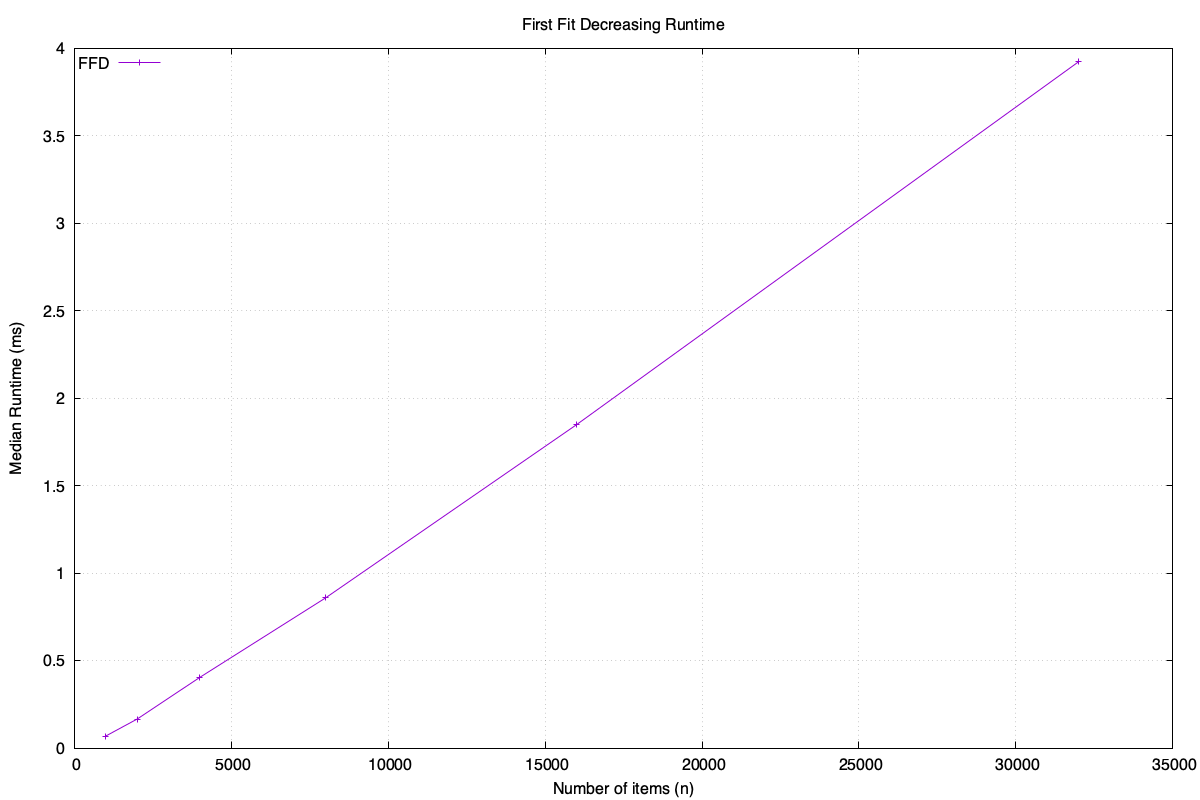
\includegraphics[width=\linewidth]{binpack_runtime.png}
\caption{Measured runtime of the First Fit Decreasing
implementation using a segment tree.}
\label{fig:binpack_runtime}
\end{figure}

The runtime increases as the number of items grows. Despite
doubling the input size at successive benchmark levels, the
observed execution times remain relatively low for the tested
instances. The implementation performs sorting in
$O(n\log n)$ time and subsequently processes each item using
segment-tree queries and updates, each requiring
$O(\log n)$ time.

Consequently, the total algorithmic runtime is
$O(n\log n)$, with $O(n)$ auxiliary storage. The measured results
are consistent with an efficient implementation of this
complexity, although empirical measurements alone cannot prove
the asymptotic bound.

\subsection{Runtime Scaling Comparison}

To further examine the scaling behavior of the Bin Packing
implementation, the measured runtime was compared with the
$n\log_2 n$ growth function.

Figure~\ref{fig:binpack_nlogn} presents this comparison.

\begin{figure}[htbp]
\centering
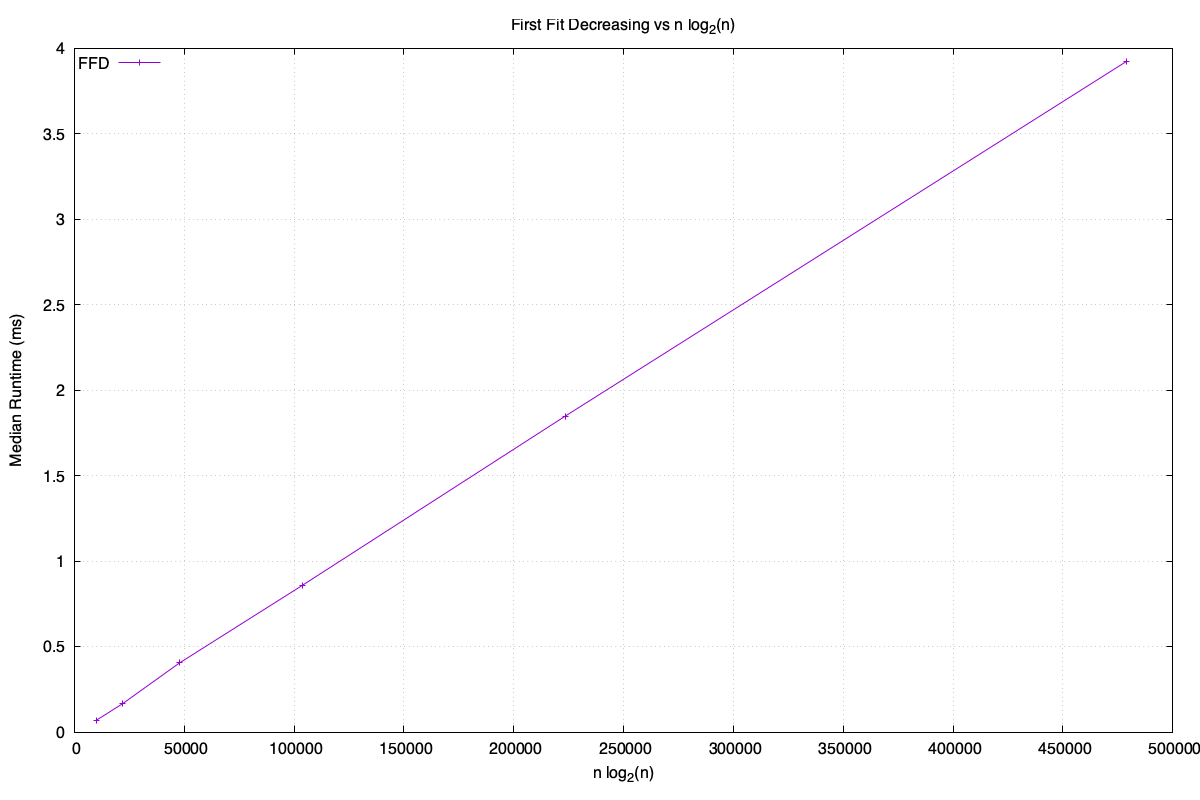
\includegraphics[width=\linewidth]{binpack_runtime_nlogn.png}
\caption{Bin Packing runtime and the $n\log_2 n$ scaling
comparison.}
\label{fig:binpack_nlogn}
\end{figure}

The comparison provides a visual reference for the expected
growth of the implementation's runtime. The $n\log_2 n$
function is used as a scaling reference rather than a direct
prediction of execution time, since it is not calibrated to the
hardware, compiler, or implementation constants.

The observed results illustrate the practical scalability of
the segment-tree-based FFD implementation over the tested input
sizes.

\section{Conclusion}

This project investigated two computational optimization problems
through established algorithmic frameworks. Water distribution
was modeled as a maximum-flow problem by introducing a
super-source and super-sink, allowing supply constraints, pipe
capacities, and demand limits to be represented within a single
flow network. Dinic's algorithm is used to compute the maximum flow
in the constructed network \cite{clrs}. The construction and correctness argument
establish that the resulting maximum-flow value corresponds
to the optimal water allocation under the assumptions of the
model.

Cloud workload consolidation was formulated as Bin Packing.
The decision problem was shown to be NP-complete through a
reduction from 3-Partition, while the optimization problem is
strongly NP-hard. To obtain practical solutions, First Fit
Decreasing was implemented with a segment tree to accelerate
the identification of the earliest feasible bin. This
implementation achieves an overall running time of
$O(n\log n)$ and auxiliary storage of $O(n)$.

The experimental results demonstrate the practical behavior
of both implementations on the tested input families.
The measured execution times increased with input size,
while the Bin Packing implementation remained efficient
across the benchmark sizes evaluated. These observations
provide empirical insight into implementation performance,
but do not replace theoretical complexity analysis.

Both models simplify their respective real-world systems.
The water-distribution model does not capture hydraulic
dynamics or pressure effects, while the Bin Packing model
does not account for multidimensional resource requirements
or operational constraints of real cloud infrastructure.
Nevertheless, these formulations demonstrate how
algorithmic modeling, reduction techniques, and efficient
implementation can be applied to meaningful optimization
problems.

\appendices
\section{LLM-Assisted Work and Disclosure}

\subsection{Tool Identification}
The project used ChatGPT (OpenAI), identified in the contemporaneous project log as GPT-6. Assistance covered project planning, formulation of the two application problems, reduction and proof drafting, C++ implementation and debugging, test design, benchmark design and interpretation, and LaTeX report preparation. The students remained responsible for reviewing and validating the submitted work.

\subsection{Prompt and Interaction Records}
The project source package contains two chronological records: \texttt{PROMPTS\_LOG.md}, which records user prompts, and \texttt{AI\_usage\_log.md}, which records relevant tool outputs, implementation work, external sources, and verification notes. The available records reproduce exact wording where it was retained. They explicitly identify earlier prompts whose exact wording was unavailable; such wording has not been reconstructed.

The following exact prompt, recorded in the AI-use log, initiated implementation:
\begin{quote}
\texttt{Yeah. that sounds like a great plan. Let's proceed with and start the project and start implementing}
\end{quote}

The following exact prompt established the continuing prompt-log requirement:
\begin{quote}
\texttt{What I want from you is to keep a log of the prompts that I have used to work on this project. Keep it stored, you can store it in a text file or some sort of file as we work through this project. Store every prompt that I gve you}
\end{quote}

The chronological prompt ledger records the assignment clarification, the email to the teaching assistant, the assistant's recorded TA clarification, project kickoff, and the prompt-logging instruction. A later addendum records prompts available from the report-completion stage. The prompt ledger is not represented as a complete export of every conversation unless the full conversation export is separately attached.

\subsection{Relevant Intermediate Results}
The recorded design process selected (i) water distribution with supply and demand limits, modeled using a super-source and super-sink in a capacitated directed network, and (ii) cloud workload consolidation modeled as one-dimensional Bin Packing. The corresponding algorithm choices were Dinic's maximum-flow algorithm and First Fit Decreasing with a max segment tree for locating the earliest bin with sufficient remaining capacity.

The retained implementation-stage output records generation of the C++ headers, command-line driver, deterministic tests, randomized comparison tests, and benchmark harness. It also records an initial CMake build and test run in the development environment. The final benchmark records contain seven timing repetitions per input size and report the median. Machine-specific measurements reported in the main paper were collected separately on the student's Apple M1 Pro machine using Apple Clang 21.0.0 and a CMake Release build.

\subsection{Verification and Responsibility}
The project was compiled and tested by the authors. The recorded tests include comparisons of Dinic against an Edmonds--Karp reference on randomized small graphs and comparisons of the segment-tree FFD implementation against a scan-based FFD reference. Benchmark measurements were collected from the submitted implementation. These checks provide implementation evidence but do not replace the mathematical proofs. The authors are responsible for the correctness of all claims, proofs, code, experimental results, and citations.

\subsection{Retained Prompt and AI-Use Logs}
The prompt ledger and AI-use log are included verbatim below as retained project records. They include exact prompts and relevant intermediate outputs where available and explicitly note archival gaps.

\lstinputlisting[caption={Chronological project prompt ledger},label={lst:prompt-ledger}]{../PROMPTS_LOG.md}
\lstinputlisting[caption={AI assistance and verification log},label={lst:ai-use-log}]{../AI_usage_log.md}

\subsection{Completeness Note}
The retained prompt ledger states that the exact wording of the original kickoff was not available in the archived conversation and therefore was not reconstructed. The AI-use log also states that its initial entry is not a substitute for full transcripts if the course requires complete transcripts. Any separately exported conversation transcripts should be included with the submission if the instructor interprets the requirement as demanding every prompt and every complete model output. No missing historical prompt or output is fabricated in this appendix.

\section{Runtime-Validation Code}\label{app:benchmark-code}

This appendix includes the C++ benchmark driver used to obtain the runtime measurements reported in Section~IV. The driver creates the benchmark inputs, performs seven timed repetitions for each size, computes the median, and writes the CSV files used for the result tables. Graph and item generation are excluded from the timed intervals. For maximum flow, construction of the Dinic network and insertion of all edges also occur before the timer; only the call to \texttt{max\_flow} is timed. For Bin Packing, the timer surrounds the complete \texttt{first\_fit\_decreasing} call, including sorting and placement.

\subsection{C++ Benchmark Driver}
The source is included directly from the project repository to avoid maintaining a duplicated code listing:
\lstinputlisting[language=C++,caption={C++ benchmark driver used to collect runtime measurements},label={lst:benchmark-driver}]{../src/benchmark.cpp}

\subsection{Reproduction Procedure}
From the project root, configure and build the Release target, execute the benchmark, and regenerate the figures using the plotting script:
\begin{lstlisting}[language=bash,caption={Reproducing the benchmark data and figures}]
cmake -S . -B build -DCMAKE_BUILD_TYPE=Release
cmake --build build --config Release
cd build
./benchmark
cd ..
gnuplot scripts/plot_benchmarks.gp
\end{lstlisting}

The benchmark writes \texttt{flow\_benchmark.csv} and \texttt{binpack\_benchmark.csv}. The graph generator and workload generator, input sizes, fixed seeds, repetition count, timing boundaries, and median calculation are visible in the included source code. The reported runtime values are machine-dependent.


\appendices
\section{LLM-Assisted Work and Disclosure}

\subsection{Tool Identification}
The project used ChatGPT (OpenAI), identified in the contemporaneous project log as GPT-6. Assistance covered project planning, formulation of the two application problems, reduction and proof drafting, C++ implementation and debugging, test design, benchmark design and interpretation, and LaTeX report preparation. The students remained responsible for reviewing and validating the submitted work.

\subsection{Prompt and Interaction Records}
The project source package contains two chronological records: \texttt{PROMPTS\_LOG.md}, which records user prompts, and \texttt{AI\_usage\_log.md}, which records relevant tool outputs, implementation work, external sources, and verification notes. The available records reproduce exact wording where it was retained. They explicitly identify earlier prompts whose exact wording was unavailable; such wording has not been reconstructed.

The following exact prompt, recorded in the AI-use log, initiated implementation:
\begin{quote}
\texttt{Yeah. that sounds like a great plan. Let's proceed with and start the project and start implementing}
\end{quote}

The following exact prompt established the continuing prompt-log requirement:
\begin{quote}
\texttt{What I want from you is to keep a log of the prompts that I have used to work on this project. Keep it stored, you can store it in a text file or some sort of file as we work through this project. Store every prompt that I gve you}
\end{quote}

The chronological prompt ledger records the assignment clarification, the email to the teaching assistant, the assistant's recorded TA clarification, project kickoff, and the prompt-logging instruction. A later addendum records prompts available from the report-completion stage. The prompt ledger is not represented as a complete export of every conversation unless the full conversation export is separately attached.

\subsection{Relevant Intermediate Results}
The recorded design process selected (i) water distribution with supply and demand limits, modeled using a super-source and super-sink in a capacitated directed network, and (ii) cloud workload consolidation modeled as one-dimensional Bin Packing. The corresponding algorithm choices were Dinic's maximum-flow algorithm and First Fit Decreasing with a max segment tree for locating the earliest bin with sufficient remaining capacity.

The retained implementation-stage output records generation of the C++ headers, command-line driver, deterministic tests, randomized comparison tests, and benchmark harness. It also records an initial CMake build and test run in the development environment. The final benchmark records contain seven timing repetitions per input size and report the median. Machine-specific measurements reported in the main paper were collected separately on the student's Apple M1 Pro machine using Apple Clang 21.0.0 and a CMake Release build.

\subsection{Verification and Responsibility}
The project was compiled and tested by the authors. The recorded tests include comparisons of Dinic against an Edmonds--Karp reference on randomized small graphs and comparisons of the segment-tree FFD implementation against a scan-based FFD reference. Benchmark measurements were collected from the submitted implementation. These checks provide implementation evidence but do not replace the mathematical proofs. The authors are responsible for the correctness of all claims, proofs, code, experimental results, and citations.

\subsection{Retained Prompt and AI-Use Logs}
The prompt ledger and AI-use log are included verbatim below as retained project records. They include exact prompts and relevant intermediate outputs where available and explicitly note archival gaps.

\lstinputlisting[caption={Chronological project prompt ledger},label={lst:prompt-ledger}]{../PROMPTS_LOG.md}
\lstinputlisting[caption={AI assistance and verification log},label={lst:ai-use-log}]{../AI_usage_log.md}

\subsection{Completeness Note}
The retained prompt ledger states that the exact wording of the original kickoff was not available in the archived conversation and therefore was not reconstructed. The AI-use log also states that its initial entry is not a substitute for full transcripts if the course requires complete transcripts. Any separately exported conversation transcripts should be included with the submission if the instructor interprets the requirement as demanding every prompt and every complete model output. No missing historical prompt or output is fabricated in this appendix.


\appendices
\section{LLM-Assisted Work and Disclosure}

\subsection{Tool Identification}
The project used ChatGPT (OpenAI), identified in the contemporaneous project log as GPT-6. Assistance covered project planning, formulation of the two application problems, reduction and proof drafting, C++ implementation and debugging, test design, benchmark design and interpretation, and LaTeX report preparation. The students remained responsible for reviewing and validating the submitted work.

\subsection{Prompt and Interaction Records}
The project source package contains two chronological records: \texttt{PROMPTS\_LOG.md}, which records user prompts, and \texttt{AI\_usage\_log.md}, which records relevant tool outputs, implementation work, external sources, and verification notes. The available records reproduce exact wording where it was retained. They explicitly identify earlier prompts whose exact wording was unavailable; such wording has not been reconstructed.

The following exact prompt, recorded in the AI-use log, initiated implementation:
\begin{quote}
\texttt{Yeah. that sounds like a great plan. Let's proceed with and start the project and start implementing}
\end{quote}

The following exact prompt established the continuing prompt-log requirement:
\begin{quote}
\texttt{What I want from you is to keep a log of the prompts that I have used to work on this project. Keep it stored, you can store it in a text file or some sort of file as we work through this project. Store every prompt that I gve you}
\end{quote}

The chronological prompt ledger records the assignment clarification, the email to the teaching assistant, the assistant's recorded TA clarification, project kickoff, and the prompt-logging instruction. A later addendum records prompts available from the report-completion stage. The prompt ledger is not represented as a complete export of every conversation unless the full conversation export is separately attached.

\subsection{Relevant Intermediate Results}
The recorded design process selected (i) water distribution with supply and demand limits, modeled using a super-source and super-sink in a capacitated directed network, and (ii) cloud workload consolidation modeled as one-dimensional Bin Packing. The corresponding algorithm choices were Dinic's maximum-flow algorithm and First Fit Decreasing with a max segment tree for locating the earliest bin with sufficient remaining capacity.

The retained implementation-stage output records generation of the C++ headers, command-line driver, deterministic tests, randomized comparison tests, and benchmark harness. It also records an initial CMake build and test run in the development environment. The final benchmark records contain seven timing repetitions per input size and report the median. Machine-specific measurements reported in the main paper were collected separately on the student's Apple M1 Pro machine using Apple Clang 21.0.0 and a CMake Release build.

\subsection{Verification and Responsibility}
The project was compiled and tested by the authors. The recorded tests include comparisons of Dinic against an Edmonds--Karp reference on randomized small graphs and comparisons of the segment-tree FFD implementation against a scan-based FFD reference. Benchmark measurements were collected from the submitted implementation. These checks provide implementation evidence but do not replace the mathematical proofs. The authors are responsible for the correctness of all claims, proofs, code, experimental results, and citations.

\subsection{Retained Prompt and AI-Use Logs}
The prompt ledger and AI-use log are included verbatim below as retained project records. They include exact prompts and relevant intermediate outputs where available and explicitly note archival gaps.

\lstinputlisting[caption={Chronological project prompt ledger},label={lst:prompt-ledger}]{../PROMPTS_LOG.md}
\lstinputlisting[caption={AI assistance and verification log},label={lst:ai-use-log}]{../AI_usage_log.md}

\subsection{Completeness Note}
The retained prompt ledger states that the exact wording of the original kickoff was not available in the archived conversation and therefore was not reconstructed. The AI-use log also states that its initial entry is not a substitute for full transcripts if the course requires complete transcripts. Any separately exported conversation transcripts should be included with the submission if the instructor interprets the requirement as demanding every prompt and every complete model output. No missing historical prompt or output is fabricated in this appendix.

\section{Runtime-Validation Code}\label{app:benchmark-code}

This appendix includes the C++ benchmark driver used to obtain the runtime measurements reported in Section~IV. The driver creates the benchmark inputs, performs seven timed repetitions for each size, computes the median, and writes the CSV files used for the result tables. Graph and item generation are excluded from the timed intervals. For maximum flow, construction of the Dinic network and insertion of all edges also occur before the timer; only the call to \texttt{max\_flow} is timed. For Bin Packing, the timer surrounds the complete \texttt{first\_fit\_decreasing} call, including sorting and placement.

\subsection{C++ Benchmark Driver}
The source is included directly from the project repository to avoid maintaining a duplicated code listing:
\lstinputlisting[language=C++,caption={C++ benchmark driver used to collect runtime measurements},label={lst:benchmark-driver}]{../src/benchmark.cpp}

\subsection{Reproduction Procedure}
From the project root, configure and build the Release target, execute the benchmark, and regenerate the figures using the plotting script:
\begin{lstlisting}[language=bash,caption={Reproducing the benchmark data and figures}]
cmake -S . -B build -DCMAKE_BUILD_TYPE=Release
cmake --build build --config Release
cd build
./benchmark
cd ..
gnuplot scripts/plot_benchmarks.gp
\end{lstlisting}

The benchmark writes \texttt{flow\_benchmark.csv} and \texttt{binpack\_benchmark.csv}. The graph generator and workload generator, input sizes, fixed seeds, repetition count, timing boundaries, and median calculation are visible in the included source code. The reported runtime values are machine-dependent.


\bibliographystyle{IEEEtran}
\bibliography{references}

\end{document}
